\documentclass[12pt]{article}
\usepackage[left=1.0in,top=1.0in,right=1.0in,bottom=1.0in]{geometry} % Document margins
\usepackage{fancyhdr}
\pagestyle{fancy}
\fancyhead[LE,LO]{Braden Anderson (203744563) \& Alan Kha (904030522)}

\usepackage[all]{xy} % for arrow diagrams.

\usepackage{authblk}
\usepackage{listings}
\usepackage{color}

% tikz stuff (for fancy flowcharts)
\usepackage{tikz}
\usetikzlibrary{shapes,arrows}
% Define block styles
\tikzstyle{decision} = [diamond, draw, fill=blue!20, 
    text width=4.5em, text badly centered, node distance=3cm, inner sep=0pt]
\tikzstyle{block} = [rectangle, draw, fill=blue!20, 
    text width=5em, text centered, rounded corners, minimum height=4em]
\tikzstyle{line} = [draw, -latex']
\tikzstyle{cloud} = [draw, ellipse,fill=red!20, node distance=3cm,
    minimum height=2em]


\definecolor{green}{rgb}{0,0.5,0}
\definecolor{purple}{rgb}{0.58,0,0.82}
\definecolor{gray}{rgb}{0.5,0.5,0.5}

\lstdefinestyle{customc}{
  belowcaptionskip=1\baselineskip,
  breaklines=true,
  frame=L,
  xleftmargin=\parindent,
  language=C,
  showstringspaces=false,
  basicstyle=\footnotesize\ttfamily,
  keywordstyle=\bfseries\color{blue},
  commentstyle=\color{green},
  identifierstyle=\color{black},
  stringstyle=\color{purple},
  numbers=left,
  numbersep=7pt,
  rulecolor=\color{black},
}

\lstset{escapechar=@,style=customc}

\begin{document}
\lstset{language=C}

\title{Lab 1ab Design Project:\\ Attack and Defend Your Shell}
\author[1]{Braden Anderson}
\affil[1]{bradencanderson@gmail.com}
\author[2]{Alan Kha}
\affil[2]{akhahaha@gmail.com}

\maketitle

\begin{abstract}
Our Lab 1ab implementation is potentially exploitable. This document will show in what ways our implementation is exploitable, and the possible forms that some exploits might take. Lastly, we will discuss security improvements that will protect against malicious attackers.
\end{abstract}

\section{Introduction}
Lab 1 implements a shell interpreter for a small subset of POSIX grammar. An input script with valid syntax is read and executed similar to the command \texttt{sh script.sh}. There are some key differences between modern shells and our own -- most notably, we do not support flow control structures such as loops, if statements, and case switches. As we will discuss in later sections, an absence of loops simplifies design concerns (and, by extension, security concerns) considerably.

\section{Security objectives}
The objective of this report is to investigate possible security flaws that a malicious user could use to attack the system running our shell. Vulnerabilities that could be used to harm the host system, in particular using a hostile input script, will be addressed. We will investigate and fix known bugs within our own program, ensuring robust behavior.


Lorem ipsum dolor sit amet, consectetur adipisicing elit, sed do eiusmod tempor incididunt ut labore et dolore magna aliqua. Ut enim ad minim veniam, quis nostrud exercitation ullamco laboris nisi ut aliquip ex ea commodo consequat. 

Duis aute irure dolor in reprehenderit in voluptate velit esse cillum dolore eu fugiat nulla pariatur. Excepteur sint occaecat cupidatat non proident, sunt in culpa qui officia deserunt mollit anim id est laborum.

\section{Overall design}
Lorem ipsum dolor sit amet, consectetur adipisicing elit, sed do eiusmod tempor incididunt ut labore et dolore magna aliqua. Ut enim ad minim veniam, quis nostrud exercitation ullamco laboris nisi ut aliquip ex ea commodo consequat. Duis aute irure dolor in reprehenderit in voluptate velit esse cillum dolore eu fugiat nulla pariatur. Excepteur sint occaecat cupidatat non proident, sunt in culpa qui officia deserunt mollit anim id est laborum.

Our shell interpreter implemenation takes a pipeline approach:

\begin{displaymath}
\xymatrix{
Shell \: script \ar[r] & \framebox{Tokenization} \ar[r] & \framebox{Parsing} \ar[r] & Execution
}
\end{displaymath}

A more detailed flowchart:

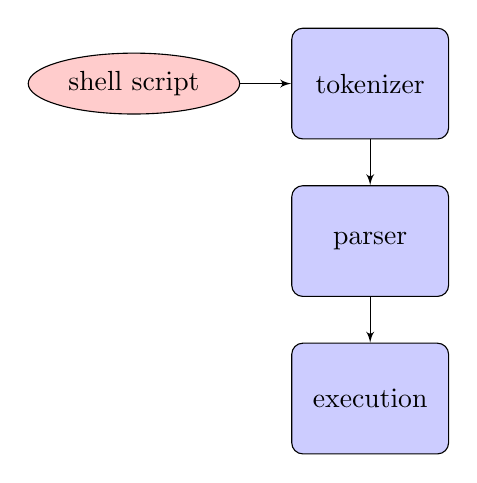
\begin{tikzpicture}[node distance = 2cm, auto]
    % Place nodes
    \node [block] (tokenizer) {tokenizer};
    \node [cloud, left of=tokenizer] (script) {shell script};
    \node [block, below of=tokenizer] (parser) {parser};
    \node [block, below of=parser] (execution) {execution};
    % Draw edges
    \path [line] (script) -- (tokenizer);
    \path [line] (tokenizer) -- (parser);
    \path [line] (parser) -- (execution);
\end{tikzpicture}

\section{Threat model}
This is where we model potential threats. This means that we use our security objectives to transform our overall application design into a system of components, data flows, and trust boundaries. Assumptions that we make:

\begin{enumerate}
  \item The shell interpreter is trusted, since we wrote all the code. However, it might enter an unsafe state.
  \item The user can be stupid or malicious.
  \item The operating system is trusted.
  \item Commands that have an interface outside our system -- for example, wget -- are potential sources of vulnerabilities.
\end{enumerate}



\section{Penetration testing}
Certain C library functions, such as printf(), gets(), and memcpy() have well-known vulnerabilities\cite{formatstring,smashingthestack}. This is because the C language does not provide builtin, high-level support for buffers or cstrings. 

Here is a program that is vulnerable to buffer overflows:
\begin{lstlisting}[frame=single]
int main(void) {
    char buf[10];
    int success = 0;
    
    printf("Enter string: \n");
    gets(buf);

    if (success)
        return 0;

    return 1;
}
\end{lstlisting}

During penetration testing we found a bug in our tokenizer where tokens can possibly include nullbytes. For example, a typical execution might take the following form:

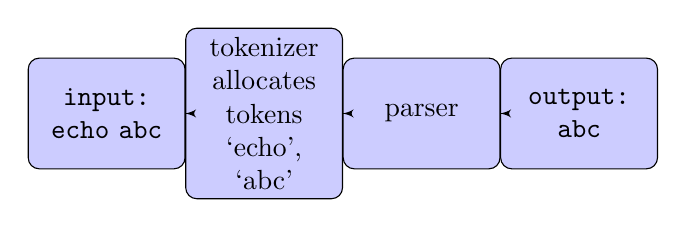
\begin{tikzpicture}[node distance = 2cm, auto]
    % Place nodes
    \node [block] (script) {\texttt{input: echo abc}};
    \node [block, right of=script] (tokenizer) {tokenizer allocates tokens `echo', `abc'};
    \node [block, right of=tokenizer] (parser) {parser};
    \node [block, right of=parser] (execution) {\texttt{output: abc}};
    % Draw edges
    \path [line] (script) -- (tokenizer);
    \path [line] (tokenizer) -- (parser);
    \path [line] (parser) -- (execution);
\end{tikzpicture}

However, we found that a word with an internal nullbyte would be improperly tokenized:

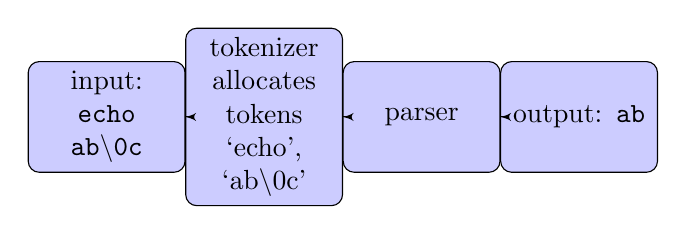
\begin{tikzpicture}[node distance = 2cm, auto]
    % Place nodes
    \node [block] (script) {input: \texttt{echo ab\textbackslash0c}};
    \node [block, right of=script] (tokenizer) {tokenizer allocates tokens `echo', `ab\textbackslash0c'};
    \node [block, right of=tokenizer] (parser) {parser};
    \node [block, right of=parser] (execution) {output: \texttt{ab}};
    % Draw edges
    \path [line] (script) -- (tokenizer);
    \path [line] (tokenizer) -- (parser);
    \path [line] (parser) -- (execution);
\end{tikzpicture}



\section{Robustness analysis}
\begin{itemize}
  \item Input validation
  \item No fixed-size buffers
  \item No calls to printf() with uncontrolled format string
  \item No unsafe library functions
\end{itemize}

\section{Challenges}

\section{Conclusion}

% This is where code samples will go.
\appendix
\section{A shellcode exploit}

\begin{thebibliography}{9}

\bibitem{formatstring}
  scut/team teso,
  Exploiting Format String Vulnerabilities.
  Stanford University,
  Version 1.2,
  2001.

\bibitem{smashingthestack}
  Aleph One,
  Smashing the Stack for Fun and Profit.
  Phrack,
  Volume 7,
  1996.
\end{thebibliography}

\end{document}
